\documentclass[letterpaper,12pt]{article}
\usepackage{amsthm,amssymb,amsmath}
\usepackage[top=25mm, bottom=25mm, left=15mm, right=15mm]{geometry}
\usepackage{graphicx}
\usepackage{array}
\usepackage{caption}
\usepackage{subcaption}
\usepackage[pagebackref=true,colorlinks,linkcolor=blue,citecolor=magenta]{hyperref}
\usepackage{fancyhdr}
\usepackage{multirow}% http://ctan.org/pkg/multirow
\usepackage{hhline}% http://ctan.org/pkg/hhline
%\settextfont[Scale=1.0]{XB Roya}
%\setlatintextfont[Scale=1.0]{XB Roya}
%\setlatintextfont[ExternalLocation,BoldFont={lmroman10-bold},BoldItalicFont={lmroman10-bolditalic},ItalicFont={lmroman10-italic}]{lmroman10-regular}
%\defpersianfont\titr[Scale=1.1]{XB Titre}
%\defpersianfont\nastaliq[Scale=1.1]{IranNastaliq}
%\defpersianfont\traffic[Scale=1]{B Traffic}
%\defpersianfont\roya[Scale=1]{XB Roya}

\def \CHWName {CPSC 525, Homework 1, Winter 2013/14}
\def \myName {Alireza Shafaei (78428133)}

\fancyhead{}
\fancyfoot{}
%\fancyhead[RO,RE]{\roya{\myName}\vspace{0.08cm}}
\fancyhead[RO,RE]{\textbf{\myName}\vspace{0.00cm}}
\fancyhead[LO,LE]{\textbf{\CHWName}\vspace{0.00cm}}
\fancyfoot[CO, CE] {\thepage}
%\fancyfoot[LO, LE] {\small{\today}}
\renewcommand{\headrulewidth}{0.3pt}
%\renewcommand{\footrulewidth}{0.3pt}
\newcommand{\threepartdef}[6]
{
	\left\{
		\begin{array}{lll}
			#1 & \mbox{ } #2 \\
			#3 & \mbox{ } #4 \\
			#5 & \mbox{ } #6
		\end{array}
	\right.
}

\newcommand{\fourpartdef}[8]
{
	\left\{
		\begin{array}{lll}
			#1 & \mbox{ } #2 \\
			#3 & \mbox{ } #4 \\
			#5 & \mbox{ } #6 \\
			#7 & \mbox{ } #8
		\end{array}
	\right.
}


\newcommand{\twopartdef}[4]
{
	\left\{
		\begin{array}{ll}
			#1 & \mbox{if } #2 \\
			#3 & \mbox{if } #4
		\end{array}
	\right.
}

\graphicspath{{./images/}}

\begin{document}
\pagestyle{fancy}

\section{Part 1}
\label{section:p1}
	For this part I used the four image set (Fig. \ref{fig:stereoeval}) on the web site of \cite{scharstein2002taxonomy}. The implementation uses the similarity measure (1) in \cite{fua1993parallel}.

\begin{figure}
        \centering
        \begin{subfigure}[b]{0.2\textwidth}
                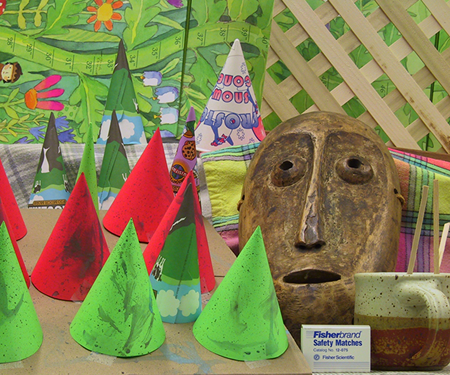
\includegraphics[width=\textwidth]{conesL.png}
%                \caption{Cones}
                \label{fig:cones}
        \end{subfigure}%
        \quad
        ~ %add desired spacing between images, e. g. ~, \quad, \qquad etc.
          %(or a blank line to force the subfigure onto a new line)
        \begin{subfigure}[b]{0.2\textwidth}
                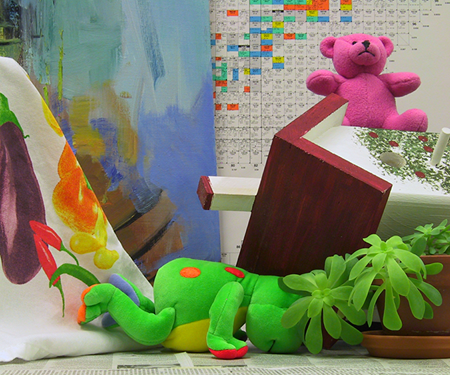
\includegraphics[width=\textwidth]{teddyL.png}
%                \caption{Teddy}
                \label{fig:teddy}
        \end{subfigure}
        \quad
        ~ %add desired spacing between images, e. g. ~, \quad, \qquad etc.
          %(or a blank line to force the subfigure onto a new line)
        \begin{subfigure}[b]{0.2\textwidth}
                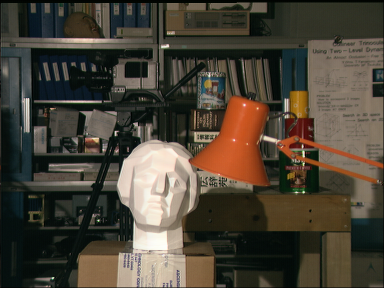
\includegraphics[width=\textwidth]{tsukubaL.png}
%                \caption{Tsukuba}
                \label{fig:tsukuba}
        \end{subfigure}
        \quad
        \begin{subfigure}[b]{0.2\textwidth}
                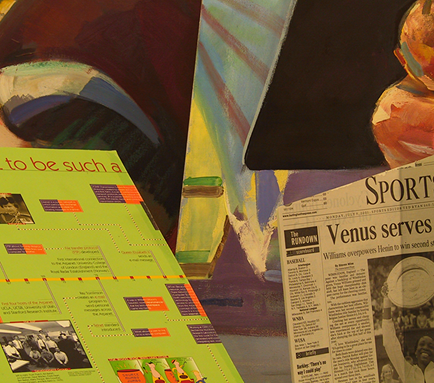
\includegraphics[width=\textwidth]{venusL.png}
%                \caption{Venus}
                \label{fig:venus}
        \end{subfigure}
        \\
        \begin{subfigure}[b]{0.2\textwidth}
                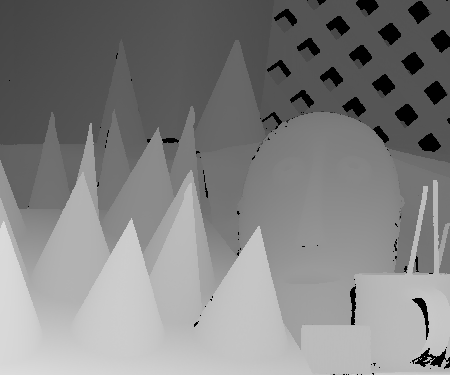
\includegraphics[width=\textwidth]{conesGT.png}
                \caption{Cones}
                \label{fig:cones}
        \end{subfigure}%
        \quad
        \begin{subfigure}[b]{0.2\textwidth}
                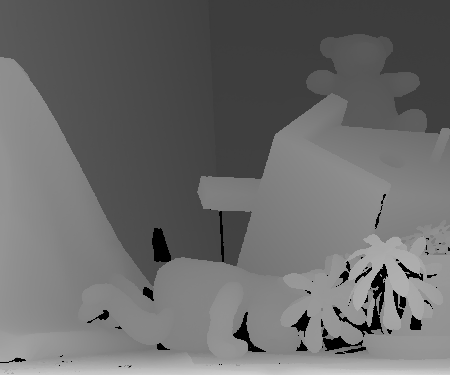
\includegraphics[width=\textwidth]{teddyGT.png}
                \caption{Teddy}
                \label{fig:teddy}
        \end{subfigure}
        \quad
        ~ %add desired spacing between images, e. g. ~, \quad, \qquad etc.
          %(or a blank line to force the subfigure onto a new line)
        \begin{subfigure}[b]{0.2\textwidth}
                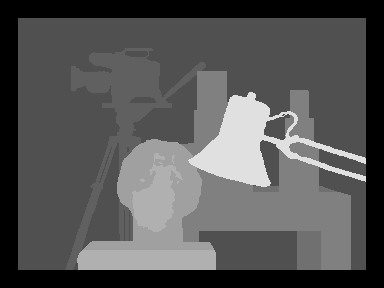
\includegraphics[width=\textwidth]{tsukubaGT.png}
                \caption{Tsukuba}
                \label{fig:tsukuba}
        \end{subfigure}
        \quad
        \begin{subfigure}[b]{0.2\textwidth}
                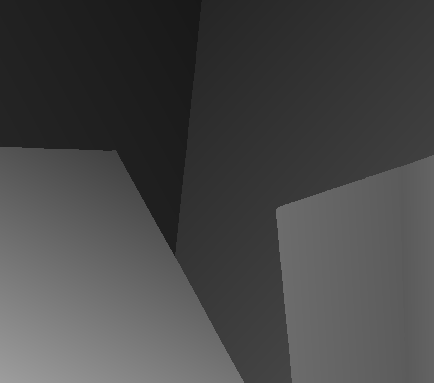
\includegraphics[width=\textwidth]{venusGT.png}
                \caption{Venus}
                \label{fig:venus}
        \end{subfigure}
        \caption{Four images and corresponding groundtruth used in \href{http://vision.middlebury.edu/stereo/}{Middlebury Stereo Evaluation}.}\label{fig:stereoeval}
\end{figure}

\subsection{Results}
	For each image of the test set I used the respective disparity range and scale (Fig \ref{fig:stereoout}).
\begin{figure}[!h]
        \centering
        \begin{subfigure}[b]{0.2\textwidth}
                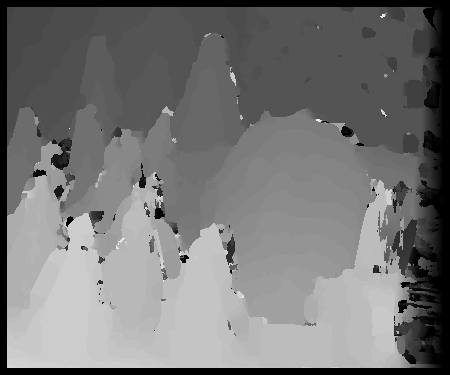
\includegraphics[width=\textwidth]{conesO.png}
        \end{subfigure}%
        \quad
        ~ %add desired spacing between images, e. g. ~, \quad, \qquad etc.
          %(or a blank line to force the subfigure onto a new line)
        \begin{subfigure}[b]{0.2\textwidth}
                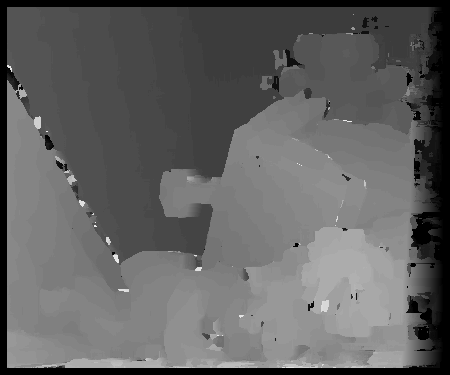
\includegraphics[width=\textwidth]{teddyO.png}
        \end{subfigure}
        \quad
        \begin{subfigure}[b]{0.2\textwidth}
                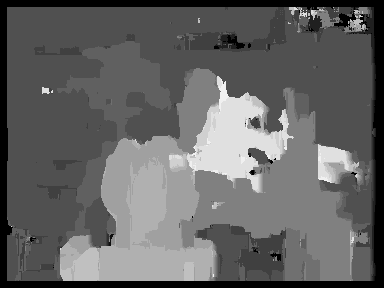
\includegraphics[width=\textwidth]{tsukubaO.png}
        \end{subfigure}
        \quad
        \begin{subfigure}[b]{0.2\textwidth}
                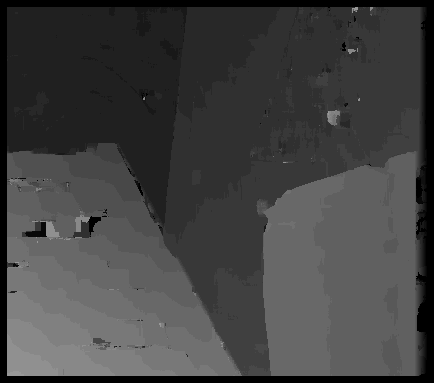
\includegraphics[width=\textwidth]{venusO.png}
        \end{subfigure}
        \caption{Preliminary results of the implemented method.}\label{fig:stereoout}
\end{figure}

\section{Part 2}
For scoring the output I compute the fraction of correct pixels within one disparity value as instructed. However, this score is determined over two different regions for each image. (i) Over all the defined groundtruth data and (ii) Non-occluded area. Doing so allows me to compare my output with state of the art methods listed at \href{http://vision.middlebury.edu/stereo/}{Middlebury Stereo Evaluation}.

\subsection{Selecting Window Size}
	To select the best window size for the similarity test I tried all the odd window sizes within range $[1, 55]$ and recorded all the scores. This parameter tuning is done on the simple approach of Part \ref{section:p1} as instructed.
	
\begin{figure}[!h]
        \centering
        \begin{subfigure}[b]{0.48\textwidth}
                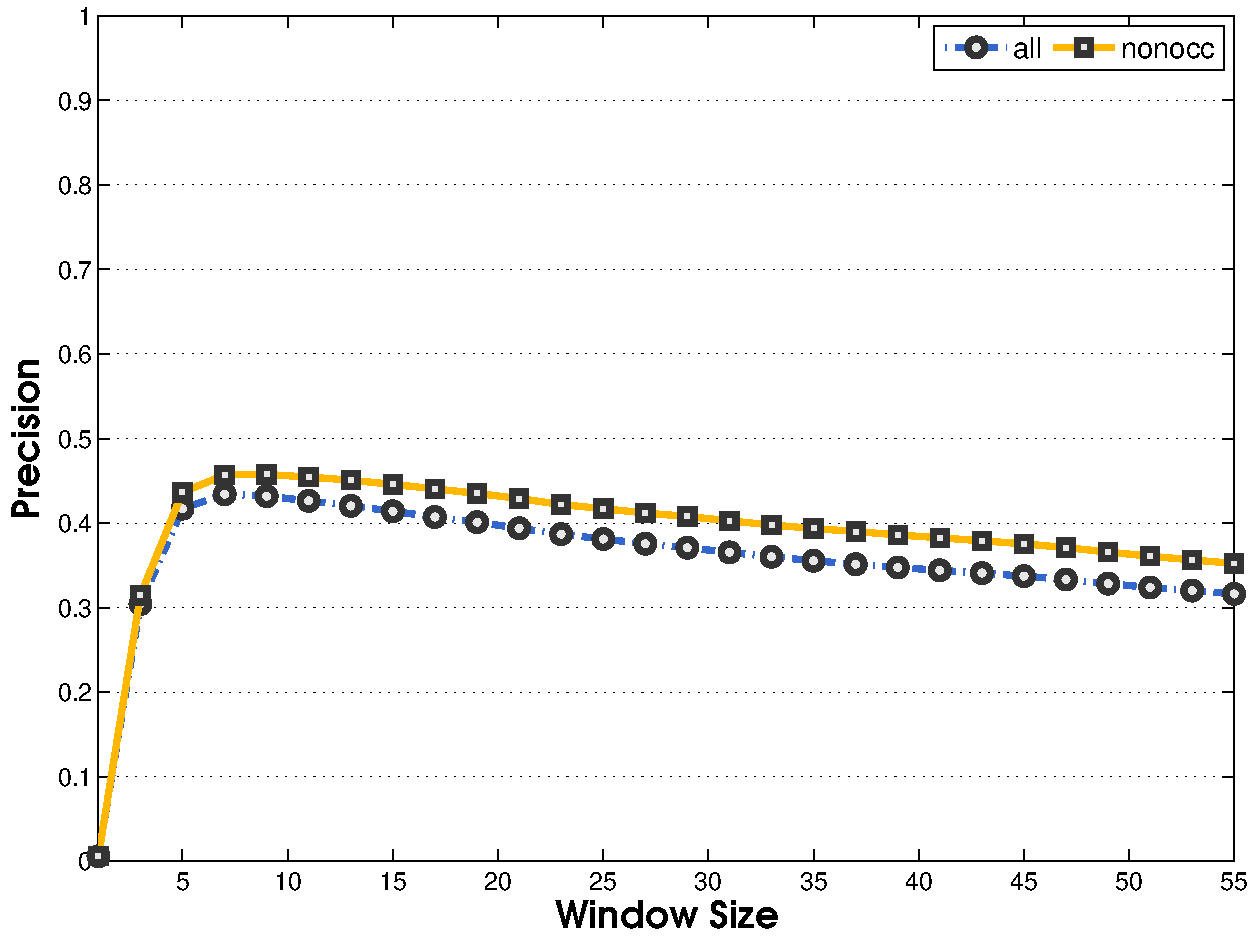
\includegraphics[width=\textwidth]{fig_w_cones.pdf}
                \caption{Cones. Best: $0.457$, window: $9\times9$}
                \label{fig:pef_cones}
        \end{subfigure}%
%        \quad
       % ~ %add desired spacing between images, e. g. ~, \quad, \qquad etc.
          %(or a blank line to force the subfigure onto a new line)
        \begin{subfigure}[b]{0.48\textwidth}
                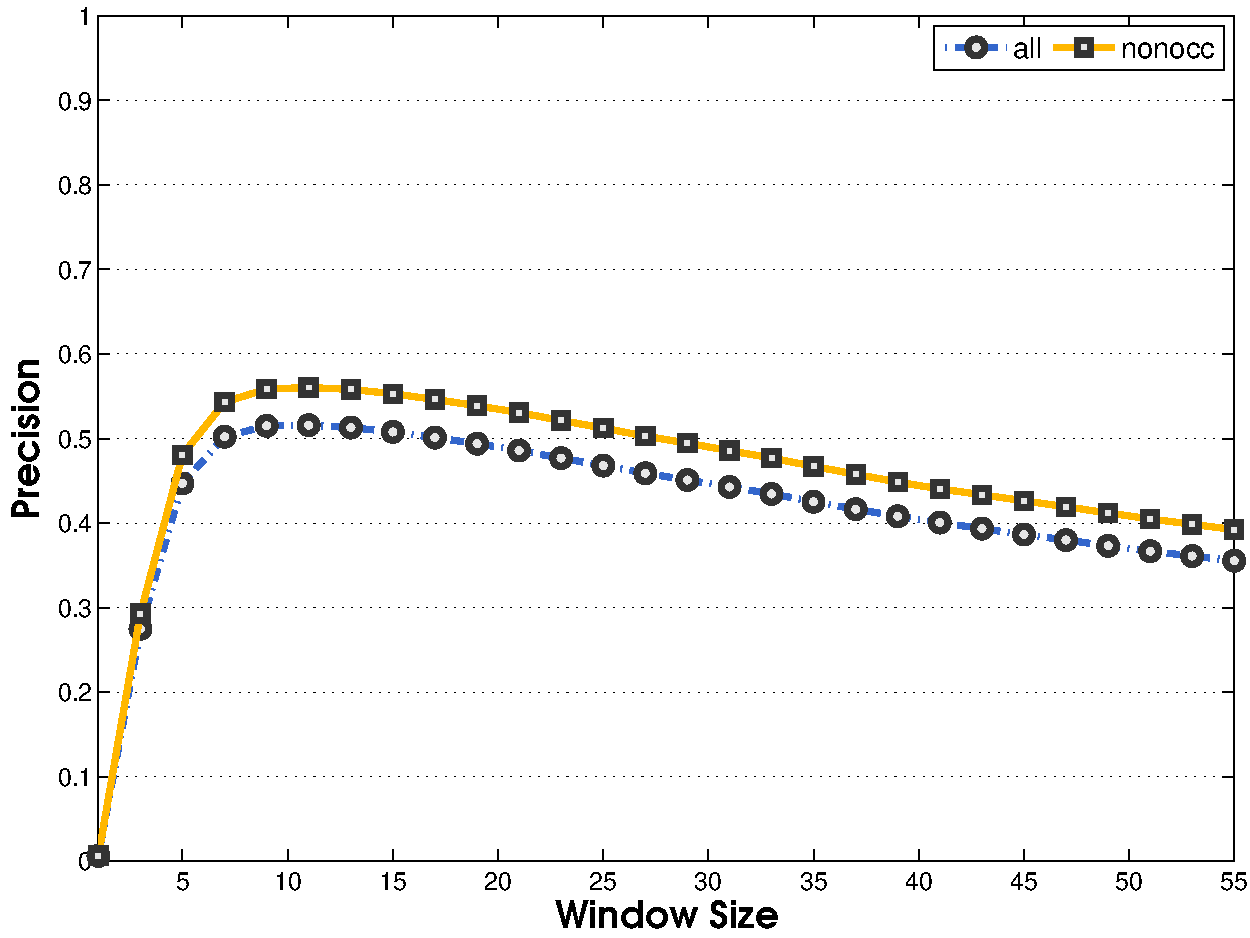
\includegraphics[width=\textwidth]{fig_w_teddy.pdf}
                \caption{Teddy. Best: $0.56$, window: $11\times11$}
                \label{fig:perf_teddy}
         \end{subfigure}
         \\
%        \quad
        \begin{subfigure}[b]{0.48\textwidth}
                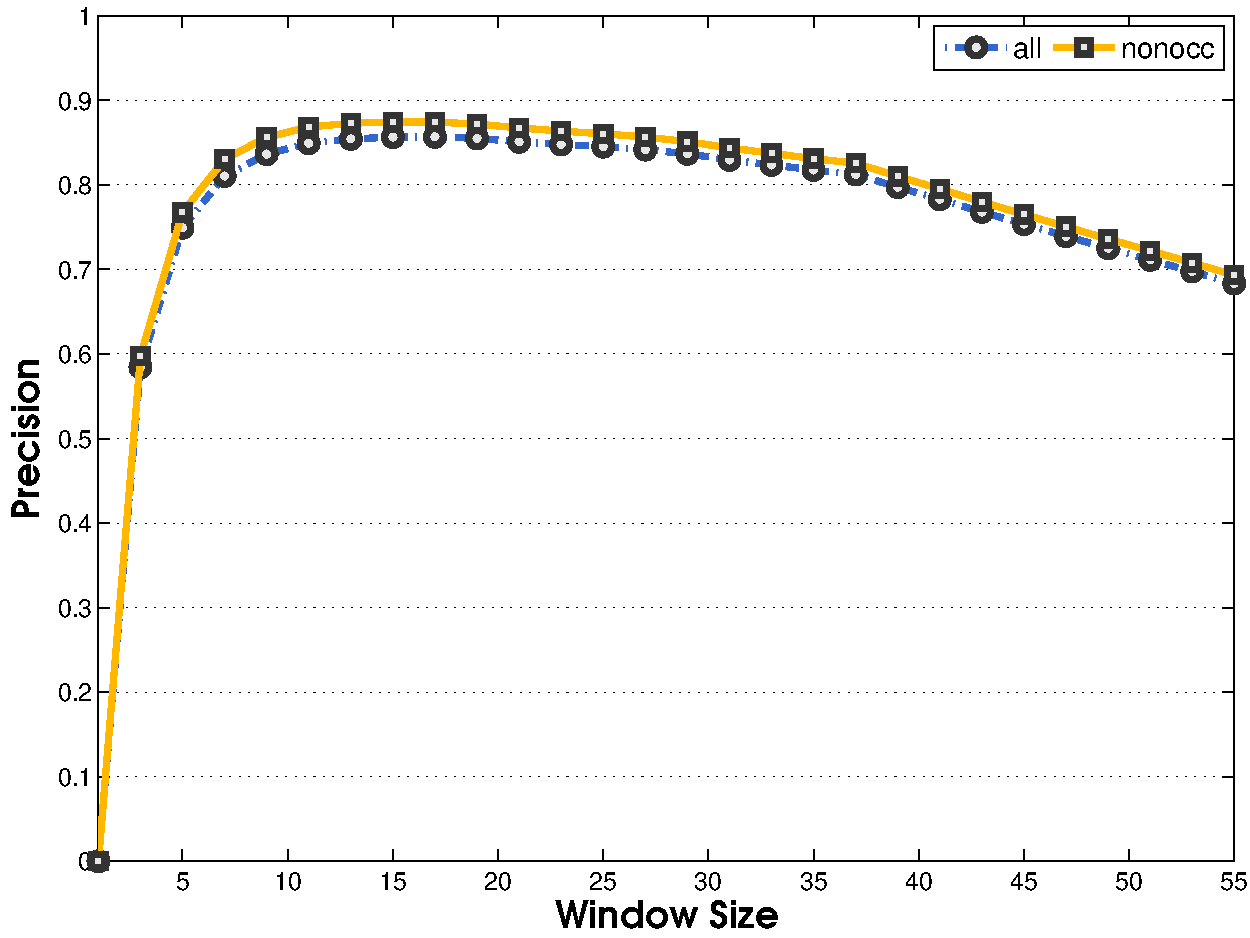
\includegraphics[width=\textwidth]{fig_w_tsukuba.pdf}
                \caption{Tsukuba. Best: $0.875$, window: $15\times15$}
        \end{subfigure}
%        \quad
        \begin{subfigure}[b]{0.48\textwidth}
                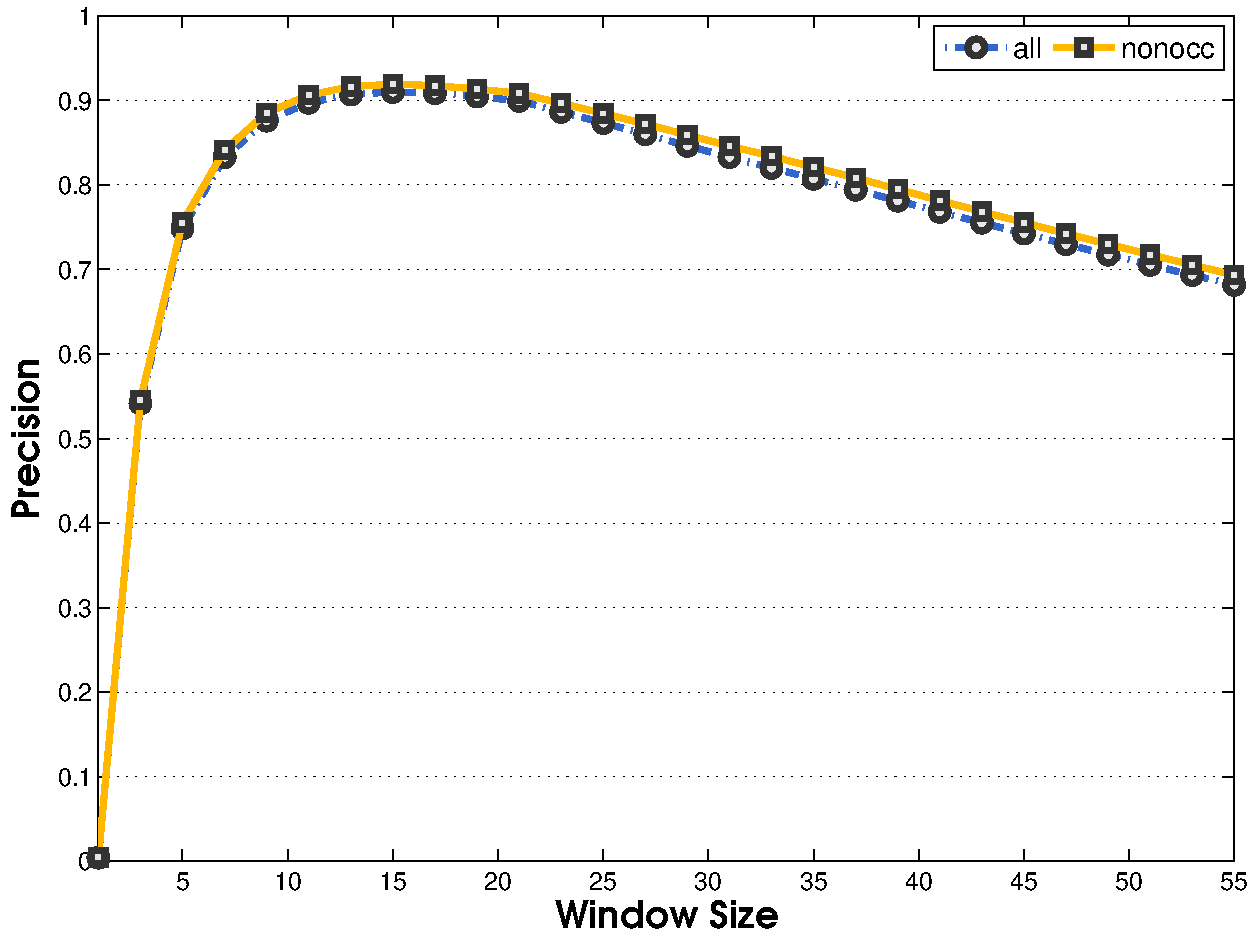
\includegraphics[width=\textwidth]{fig_w_venus.pdf}
                \caption{Venus. Best: $0.919$, window: $15\times15$}
        \end{subfigure}
        \caption{Precision of the implementation as a function of window size.}\label{fig:graphs}
\end{figure}

As you can see in Fig. \ref{fig:graphs}, setting the window size to $15$ is a reasonable decision as it approximately maximizes the average precision. (For more images see Fig. \ref{fig:more})

Given that our implementation has a significantly worse performance on \ref{fig:pef_cones} and \ref{fig:perf_teddy} you may wonder what's the explanation for this. To answer this question I cut the regions of the images which were incorrectly labeled. The results are shown in figure \ref{fig:cut}.

\begin{figure}[!h]
        \centering
        \begin{subfigure}[b]{0.30\textwidth}
                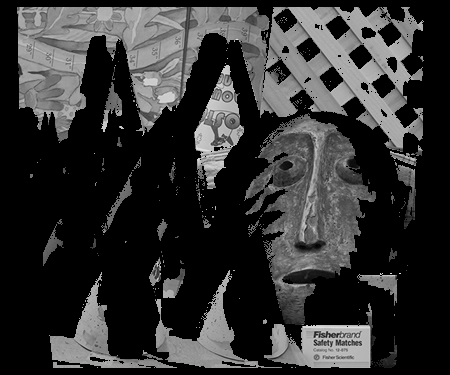
\includegraphics[width=\textwidth]{correct-conesO.png}

        \end{subfigure}%
        \quad
       % ~ %add desired spacing between images, e. g. ~, \quad, \qquad etc.
          %(or a blank line to force the subfigure onto a new line)
        \begin{subfigure}[b]{0.30\textwidth}
                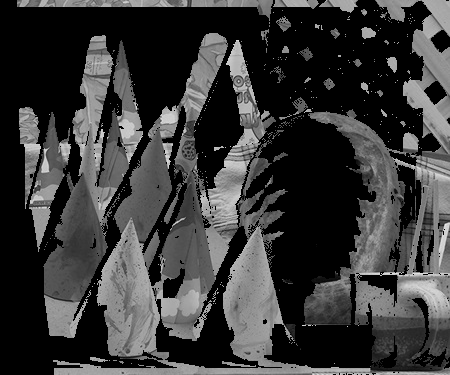
\includegraphics[width=\textwidth]{icorrect-conesO.png}

         \end{subfigure}
         \\
        \begin{subfigure}[b]{0.30\textwidth}
                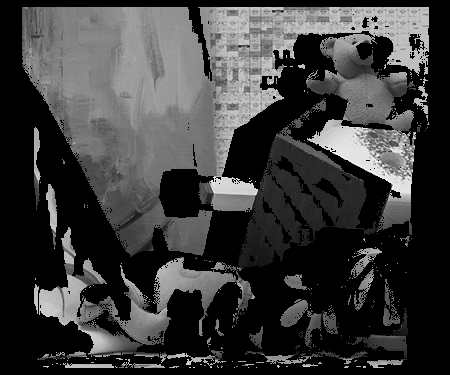
\includegraphics[width=\textwidth]{correct-teddyO.png}

        \end{subfigure}%
        \quad
       % ~ %add desired spacing between images, e. g. ~, \quad, \qquad etc.
          %(or a blank line to force the subfigure onto a new line)
        \begin{subfigure}[b]{0.30\textwidth}
                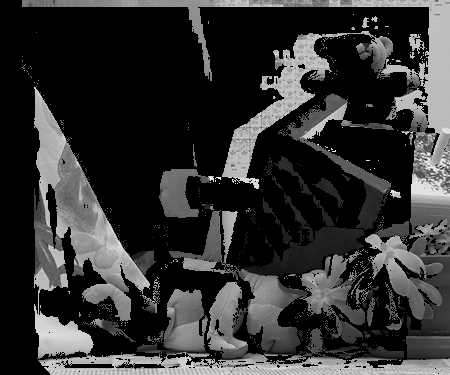
\includegraphics[width=\textwidth]{icorrect-teddyO.png}

         \end{subfigure}
         \\
        \begin{subfigure}[b]{0.30\textwidth}
                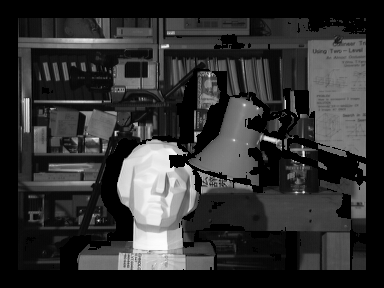
\includegraphics[width=\textwidth]{correct-tsukubaO.png}

        \end{subfigure}%
        \quad
       % ~ %add desired spacing between images, e. g. ~, \quad, \qquad etc.
          %(or a blank line to force the subfigure onto a new line)
        \begin{subfigure}[b]{0.30\textwidth}
                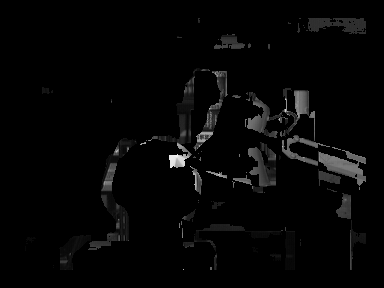
\includegraphics[width=\textwidth]{icorrect-tsukubaO.png}

         \end{subfigure}
         \\
        \begin{subfigure}[b]{0.30\textwidth}
                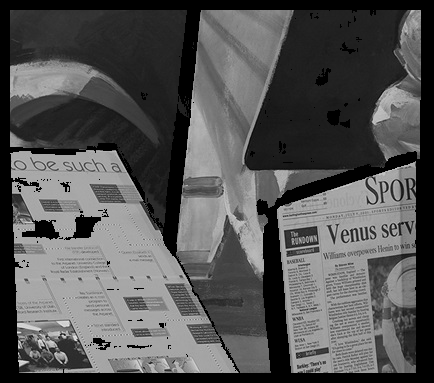
\includegraphics[width=\textwidth]{correct-venusO.png}

        \end{subfigure}%
        \quad
       % ~ %add desired spacing between images, e. g. ~, \quad, \qquad etc.
          %(or a blank line to force the subfigure onto a new line)
        \begin{subfigure}[b]{0.30\textwidth}
                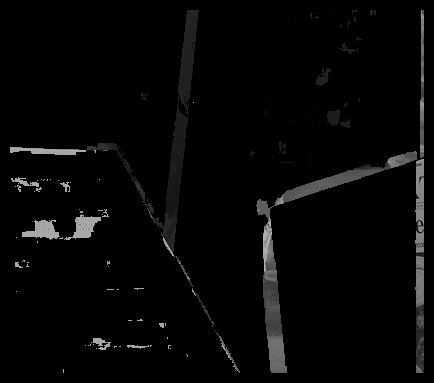
\includegraphics[width=\textwidth]{icorrect-venusO.png}

         \end{subfigure}
        \caption{Left images are the correctly labeled portions and right images are incorrectly labeled portions of the image}\label{fig:cut}
\end{figure}

Based on the images of Fig. \ref{fig:cut} I can think of two possible reoccurring patterns that appear in the error images.

\begin{itemize}
	\item \textbf{Non-Distinctive Pattern.} Most of the error regions in Teddy and Cones have a reoccurring pattern that magnifies the weakness of our approach for similarity testing. In such circumstances, we also need to rely on the geometric displacements in neighboring pixels.
	\item \textbf{Boundary Regions.} This type of errors usually appear when we're around object boundaries and thus unable to correctly identify the matching region.
\end{itemize}

Furthermore, I analyzed the distance of first best match to second best match to examine the helpfulness of our similarity measure. The following graphs show the ratio $\frac{1-NCC_{best}}{1-NCC_{second best}}$ for when we have found the correct match and for when we are wrong.

\begin{figure}[!h]
        \centering
        \begin{subfigure}[b]{0.48\textwidth}
                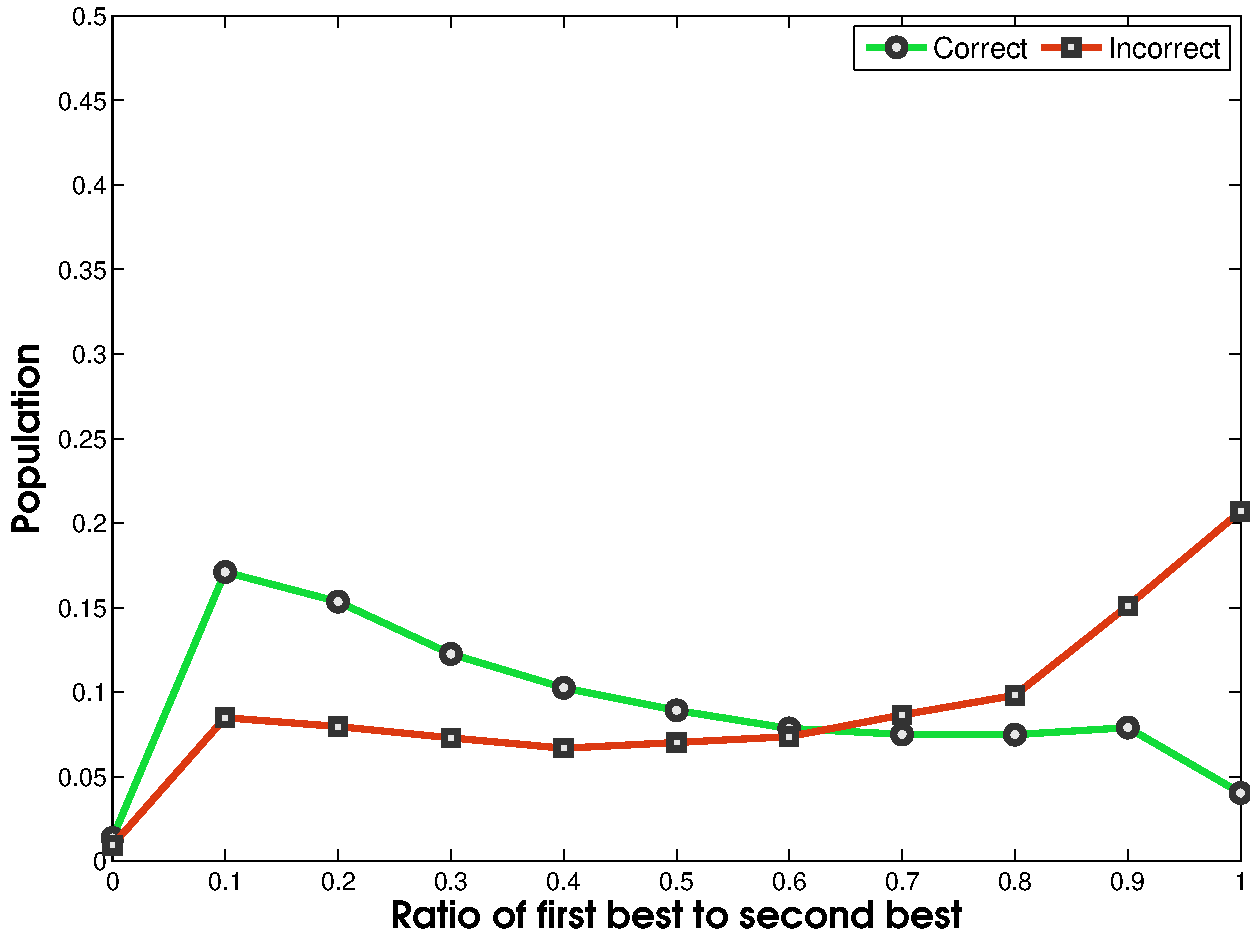
\includegraphics[width=\textwidth]{rat_w_cones.pdf}
                 \caption{Cones.}
               % \label{fig:pef_cones}
        \end{subfigure}%
%        \quad
       % ~ %add desired spacing between images, e. g. ~, \quad, \qquad etc.
          %(or a blank line to force the subfigure onto a new line)
        \begin{subfigure}[b]{0.48\textwidth}
                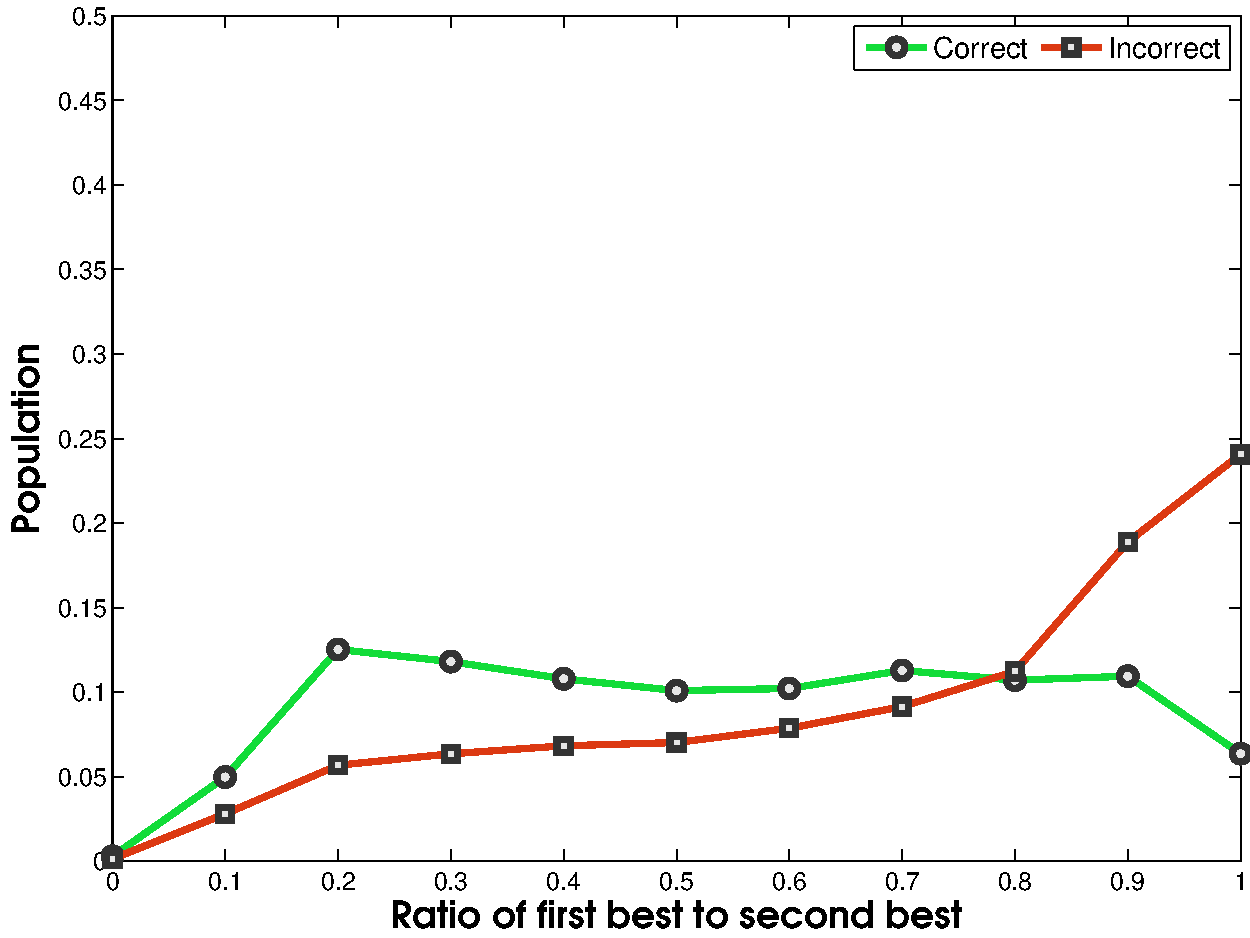
\includegraphics[width=\textwidth]{rat_w_teddy.pdf}
                \caption{Teddy.}
              %  \label{fig:perf_teddy}
         \end{subfigure}
         \\
%        \quad
        \begin{subfigure}[b]{0.48\textwidth}
                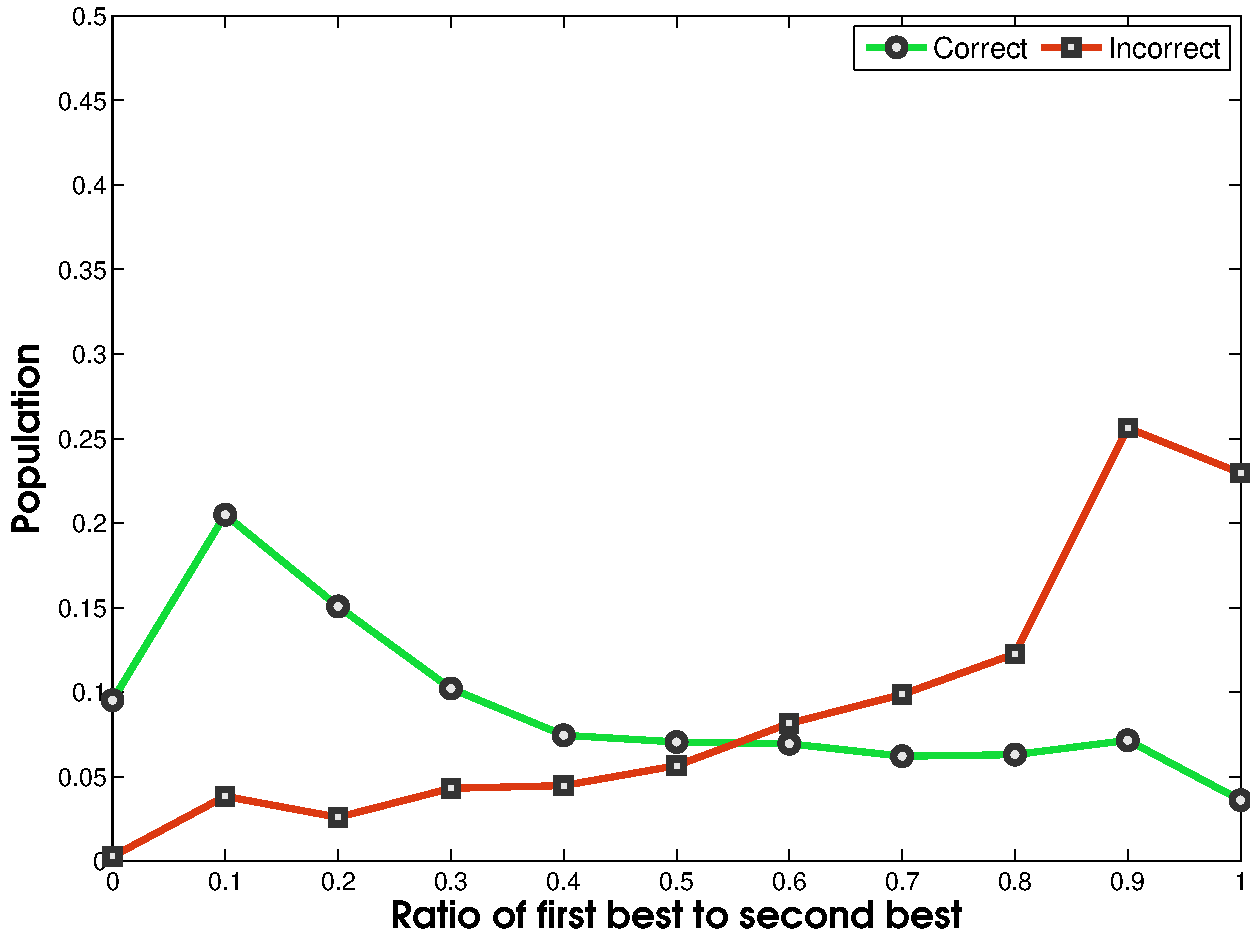
\includegraphics[width=\textwidth]{rat_w_tsukuba.pdf}
                \caption{Tsukuba.}
        \end{subfigure}
%        \quad
        \begin{subfigure}[b]{0.48\textwidth}
                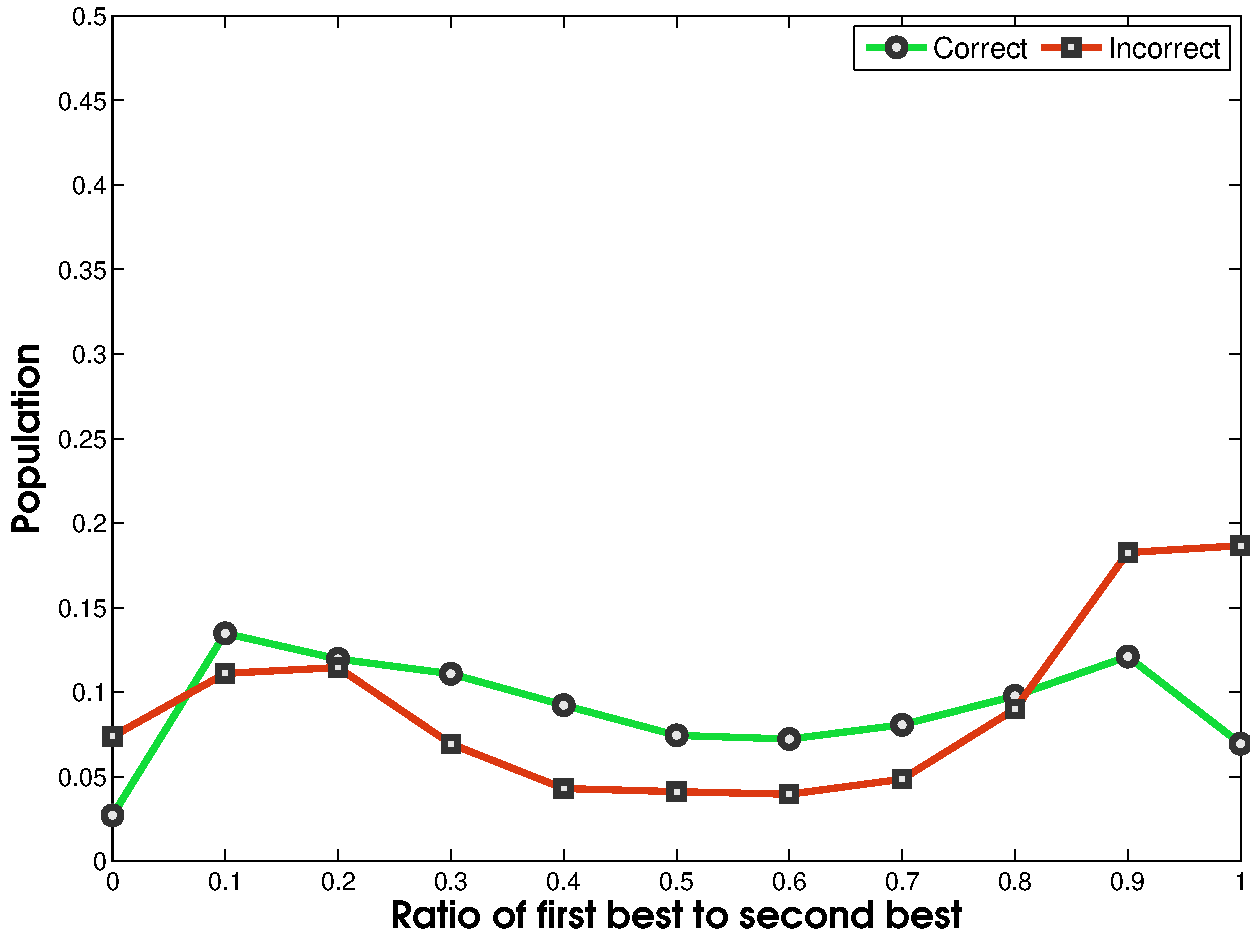
\includegraphics[width=\textwidth]{rat_w_venus.pdf}
                \caption{Venus.}
        \end{subfigure}
        \caption{The ratio of distances of first match and second match from the best possible match ($NCC=1$).}
        \label{fig:rat}
\end{figure}

Based on the Fig. \ref{fig:rat}, we can perform validation check by marking estimations with ratios over $0.8$ as bad estimations (similar to double peek test discussed in the class). It must be noted that it is equally important to correctly fill the marked regions, or the final outcome could be even worse as we're also marking a small portion of the correctly estimated region as wrong.

\section{Part 3}
For this part, I implemented the validity check described before and tried two methods to fill the marked region.
\begin{itemize}
	\item \textbf{Nearest Valid.} In this approach each marked region is filled with the value of nearest valid region.
	\item \textbf{Linear Row Interpolation.} After identifying the maximal length marked region in each row of the image, that area is linearly interpolated.
\end{itemize}

\begin{table}[!h]
	\centering
	\caption{Results for different filling methods. The window size used for evaluation is $15\times15$ and the error in non-occluding region is reported.}
	\begin{tabular}{|c|c||c|c||c|}
	\hline
Filling	Method & Image & Without & With & Change \\
	\hline
	\multirow{4}{*}{Nearest Valid}	& Cones & 0.446 & \textbf{0.453} & +0.007\\
	& Teddy & 0.553 & \textbf{0.56} & +0.007\\
	& Tsukuba & 0.875 & \textbf{0.895} & +0.02\\
	& Venus & 0.919 & \textbf{0.924} & +0.005\\
	\hline 
	\multirow{4}{*}{Linear Row Interpolation}	& Cones & 0.446 & \textbf{0.477} & +0.031\\
	& Teddy & 0.553 & \textbf{0.577} & +0.024\\
	& Tsukuba & 0.875 & \textbf{0.891} & +0.016\\
	& Venus & 0.919 & \textbf{0.923} & +0.004\\
	\hline 
	\end{tabular}
\end{table}

\begin{figure}[!h]
        \centering
        \begin{subfigure}[b]{0.30\textwidth}
                \includegraphics[width=\textwidth]{ConesO.png}
                 \caption{Cones without validity check.}
               % \label{fig:pef_cones}
        \end{subfigure}%
        \quad
        \begin{subfigure}[b]{0.30\textwidth}
                \includegraphics[width=\textwidth]{ConesOcv.png}
                 \caption{Cones with nearest valid.}
               % \label{fig:pef_cones}
        \end{subfigure}%
        \quad
       % ~ %add desired spacing between images, e. g. ~, \quad, \qquad etc.
          %(or a blank line to force the subfigure onto a new line)
        \begin{subfigure}[b]{0.30\textwidth}
                \includegraphics[width=\textwidth]{ConesOli.png}
                \caption{Cones with lin. interpolation.}
              %  \label{fig:perf_teddy}
         \end{subfigure}
\        \caption{Output after filling the identified invalid region with different methods.}
        \label{fig:rat}
\end{figure}

Interestingly the linearly interpolated image, though less visually appealing, gives a better estimation compared to the smooth looking output of the nearest valid method.

The overall performance improvement of methods based on the proposed validity check is not expected to be significant, mainly because the correct and incorrect region in Fig. \ref{fig:rat}, except for Tsukuba, can't be well distinguished.
\newpage
\section{More Images}

\begin{figure}[!h]
\centering
	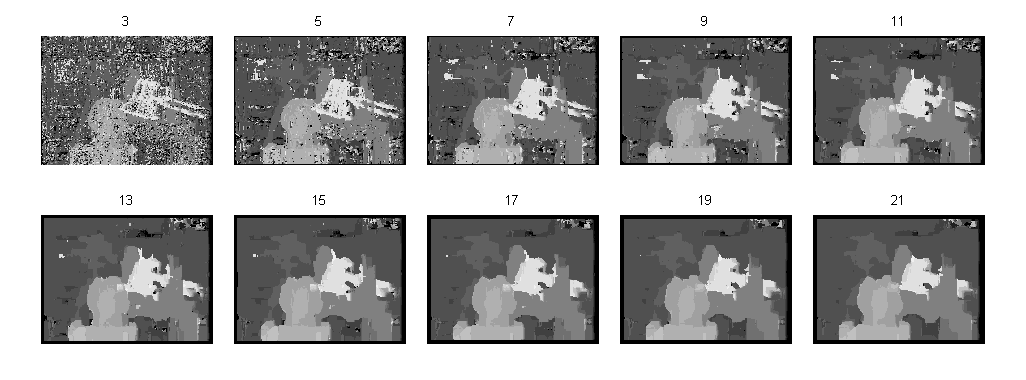
\includegraphics[width=19cm]{samples2.png}
	\caption{Tsukuba image with different window sizes.}
	\label{fig:more}
\end{figure}


\bibliographystyle{apalike}
\bibliography{ref}

\end{document}
